As Larry Garfield explains in \cite[]{pac-vs-mvc} Drupal uses the architectural pattern PAC\footnote{Presentation Abstraction Control - \url{http://en.wikipedia.org/wiki/Presentation-abstraction-control}} for organising its structure and functionality.  The PAC pattern is less known and used than the architectural pattern MVC\footnote{Model View Controller - \url{http://martinfowler.com/eaaDev/uiArchs.html}}.  The new Land Portal tries to transform the PAC pattern to work in a way more similar to the MVC pattern.

In this tutorial we will explain how to create a custom view and include it in the new Land Portal.  Those three steps are required and will be explained in detail.
\begin{enumerate}
	\item Create the entry in the routes configuration file
	\item Create the model that returns the required data
	\item Create the view to show the data returned by the model
\end{enumerate}

Before taking the following steps it is recommended to take a look at the structure of the \textit{LandPortal uris} module (section \ref{vista_landportal_uris}, chapter \ref{chapter05}) and the activity of the custom templates rendering (section \ref{actividad:landportal-uris_theme}, chapter \ref{chapter05}).

\subsection{Creating the route}
	The first step to create a custom view is to create the route under the users will access the view.  The routes are declared in the \textit{routes.json} file.  This file is stored in the path \textit{DRUPAL\_HOME/sites/all/modules/custom/modules/landportal\_uris/routes.json}.
	
	The image \ref{fig:rutas_ejemplo} shows some entries of the \textit{routes.json} file.  Each entry has the following fields:
	\begin{itemize}
		\item
			\textbf{Path}  The path specifies the URL of the view.  The path is always relative to the main Drupal URL.  To specify a \textit{wildcard} use a \% symbol.  For example, in the image \ref{fig:rutas_ejemplo} the path \textit{book/regions/\%} will match the URLs \textit{book/regions/1}, \textit{book/regions/150}, etc
		
		\item
			\textbf{Name} The name is used to retrieve the corresponding model and view.  The name \textit{regions} will look for the model \textit{Regions} and the view \textit{regions.mustache}.
			
		\item
			\textbf{Title} The title is printed in the browser tab in which the user loads the template.
		
		\item
			\textbf{Navigation}  The navigation sets the tab that will be selected in the header bar when te user loads the template.
		\item
			\textbf{Params}  The params specify which parameters will be taken from the URL and passed to the model.  The parameter corresponds to the position of the \textit{wildcard} in the \textit{path}, the position starts in 0. For example, in the image \ref{fig:rutas_ejemplo} the path \textit{book/regions/\%} has the \textit{wildcard} in the position 2, being the position 0 \textit{book} and the position 1 \textit{regions}.  If a path does not receive any arguments leave the parameters empty.
		\item
			\textbf{Redirect}  Apart from the previous fields, an entry in the routes file may have a \textit{redirect} field.  This field contains a path that will be loaded automatically.  For example, in the image \ref{fig:rutas_ejemplo} the path \textit{book} will redirect to the path \textit{book/regions}.  When the \textit{redirect} field is present, the fields \textit{navigation} and \textit{params} can be omitted.
	\end{itemize}
	
	\begin{figure}[h]
		\centering
		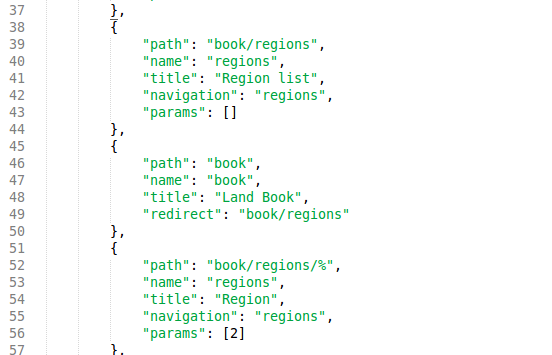
\includegraphics[width=11cm]{custom_view/routes_example}
		\caption{Snippet of the \textit{routes.json} file content}
		\label{fig:rutas_ejemplo}
	\end{figure}
	
The image \ref{fig:rutas_nueva} shows a custom created route for this tutorial.  The route will be accessible in the path \textit{helloworld} and will load the model \textit{helloworld.php} and the template \textit{helloworld.mustache}.  In the following sections we will see how to create the model and the template.
	\begin{figure}[h]
		\centering
		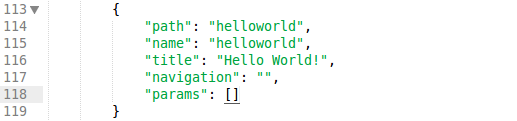
\includegraphics[width=10cm]{custom_view/routes_new}
		\caption{Example of new entry in the \textit{routes.json} file}
		\label{fig:rutas_nueva}
	\end{figure}

\subsection{Creating the model}
	The second step to create a custom view is to create a model.  The models return the data that is shown to the user by the template.  The models are created in the directory \textit{DRUPAL\_HOME/sites/all/modules/custom/modules/landportal\_uris/models/}.  The model will be automatically loaded by its name.
	
	In the image \ref{fig:rutas_nueva} we created a new path to make a custom template.  The path had the name \textit{helloworld}, so our model will have the name \textit{helloworld.php} in order to be automatically loaded by Drupal.
	
	The image \ref{fig:rutas_modelo} shows the content of our new model.  Every model must have two basic characteristics in order to be correctly loaded by Drupal:
	\begin{itemize}
		\item
			The class name of the model must be the same as the file name, but with the first letter upercase.  Our model file was called \textit{helloworld.php} so the model's class must be called \textit{Helloworld}.
		\item
			Every model must have a method \textit{get} that returns an array with the contents to populate the template.  In this case the model returns a single key called \textit{name}, which will be rendered in the template.
	\end{itemize}
	
	\begin{figure}[h]
		\centering
		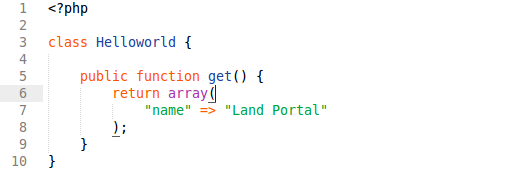
\includegraphics[width=10cm]{custom_view/model_example}
		\caption{Example of the model class in the \textit{helloworld.php} file}
		\label{fig:rutas_modelo}
	\end{figure}

\subsection{Creating the template}
	The final step to create a custom view is to create the template that will be rendered to the user.  The templates are created in the directory \textit{DRUPAL\_HOME/sites/all/themes/book/views/}.  The template will be automatically load by its name.
	
	In the image \ref{fig:rutas_nueva} we created a new path to make a custom template.  The path had the name \textit{helloworld}, so our template will have the name \textit{helloworld.mustache} in order to be automatically loaded by Drupal.  
	
	The templates are created using \textit{mustache}\footnote{It is not the object of this tutorial to explain \textit{mustache} and it syntaxis.  For more details about how \textit{mustache} works, take a look at the official documentation in \url{http://mustache.github.io/}}.  The arguments between the mustaches (\{\{ and \}\}) will be automatically replaced by its value before the template is rendered to the user.
	
	The image \ref{fig:rutas_mustache} shows the contents of our custom template in the file \textit{helloworld.mustache}.  The model that we created in the image \ref{fig:rutas_modelo} returned a key named \textit{name} that we will use in the template.
	
	The image \ref{fig:rutas_resultado} shows the result of the view that we have created in this tutorial.  As you can see, the path corresponds to the one specified in the image \ref{fig:rutas_nueva}, and the mustaches in the image \ref{fig:rutas_mustache} have been substituted by the data returned from the model (image \ref{fig:rutas_modelo}).
	\begin{figure}[h]
		\centering
		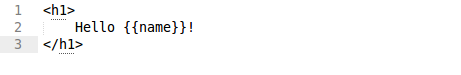
\includegraphics[width=10cm]{custom_view/template_example}
		\caption{Example of the template in the \textit{helloworld.mustache} file}
		\label{fig:rutas_mustache}
	\end{figure}
	
	\begin{figure}[h]
		\centering
		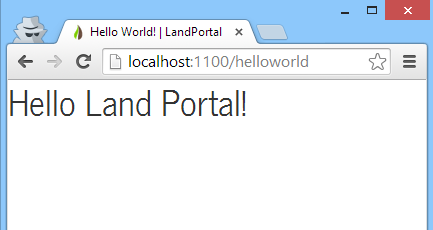
\includegraphics[width=10cm]{custom_view/result}
		\caption{Result of the custom view}
		\label{fig:rutas_resultado}
	\end{figure}